\chapter{Results}
\label{chapter:Results}

The final output of this work is twofold - an evaluation of support vector machines and ensemble learning methods in the domain of text classification, and a web based interface that implements the evaluated techniques and presents a system that can monitor the public feed from the Internet to find out people who are suffering emotional distress and may need help.

\section{Evaluation}
\label{section:evaluation}
The evaluation of all algorithms is done on the comments dataset \cite{kaggle}. Scores from normal supervised learning and online supervised learning are calculated and presented. To report online learning scores, the learning continues in iterations. In each iteration, 100 more random samples are picked on which the models are trained and the accuracy is measured. This is continued until no more samples are left. While this does not conform precisely to the definition of online learning, this approach is still used because of two reasons. First, this is very similar to how the classifiers in the system are updated each time there is new training data available. Second, in the most elementary approach for online learning, a new and updated classifier is obtained by retraining on the support vectors from the original classifier and the new sample. Under the experimental settings for the problem at hand, this approach yielded very poor results which could not be used to implement the final system. All accuracies reported henceforth are calculated using 10-fold cross-validation, training the model on 90\% of the data and testing on the remaining 10\%, and repeating this process 10 times to get the average of all 10 measurements.

\subsection{Support Vector Machine}
The behavior of support vector machine based classification depends heavily on the kernel being used. Using a linear kernel yields a cross validation accuracy of 79.06\%, while using either of polynomial/RBF/sigmoid kernels gives an accuracy of only 34.39\%. This can be attributed to the notion of how kernel functions operate. A kernel function calculates the similarity between two vectors when the vectors have been transformed from their original low dimensional space into a high dimensional space. In the current scenario, the text corpus contains 23175 features, which is already a very high number. Any transformation from this space into an even higher space results in a decrease in the final accuracy calculated, as can be noted in the results.\\

When using a linear kernel, the accuracy of an SVM shows an increase as the number of input instances increases. The score ranges from 67.00\% when measuring on 100 samples, to 79.35\% when measuring on 5800 samples, as shown in Figure~\ref{fig:svm_accuracy}.\\

\begin{figure}
    \centering
    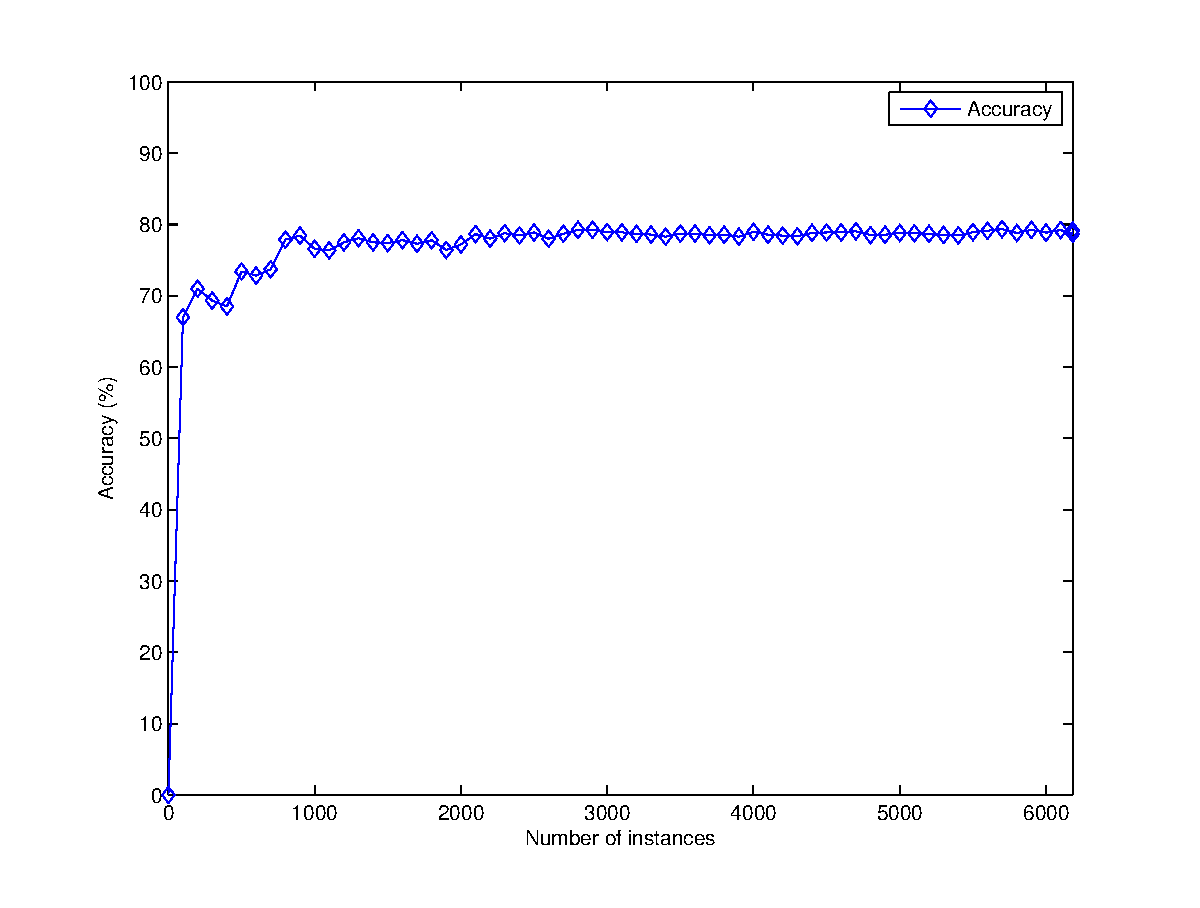
\includegraphics[width=0.8\textwidth]{svm_accuracy.eps}
    \caption{Accuracy of a linear kernel support vector machine, measured against the total number of instances}
    \label{fig:svm_accuracy}
\end{figure}

Support vectors is a term for the subset of data points that the main classifier uses to establish the margin between the two class of points. Measuring the number of support vectors against the total number of instances gives an idea about the performance of the classifier - the more the number of support vectors (relative to the number of instances), the harder it is to perform a classification. Figure~\ref{fig:svm_n_sv} shows this variation for the problem at hand. The number ranges from 90 for 100 samples to 3771 for 6182 samples, the increase being almost linear in the number of instances. It can be noted that the ratio of support vectors to the total number of points decreases from 0.9 to around 0.6, which shows that the more the information available to the classifier, the easier the task at hand becomes.

\begin{figure}
    \centering
    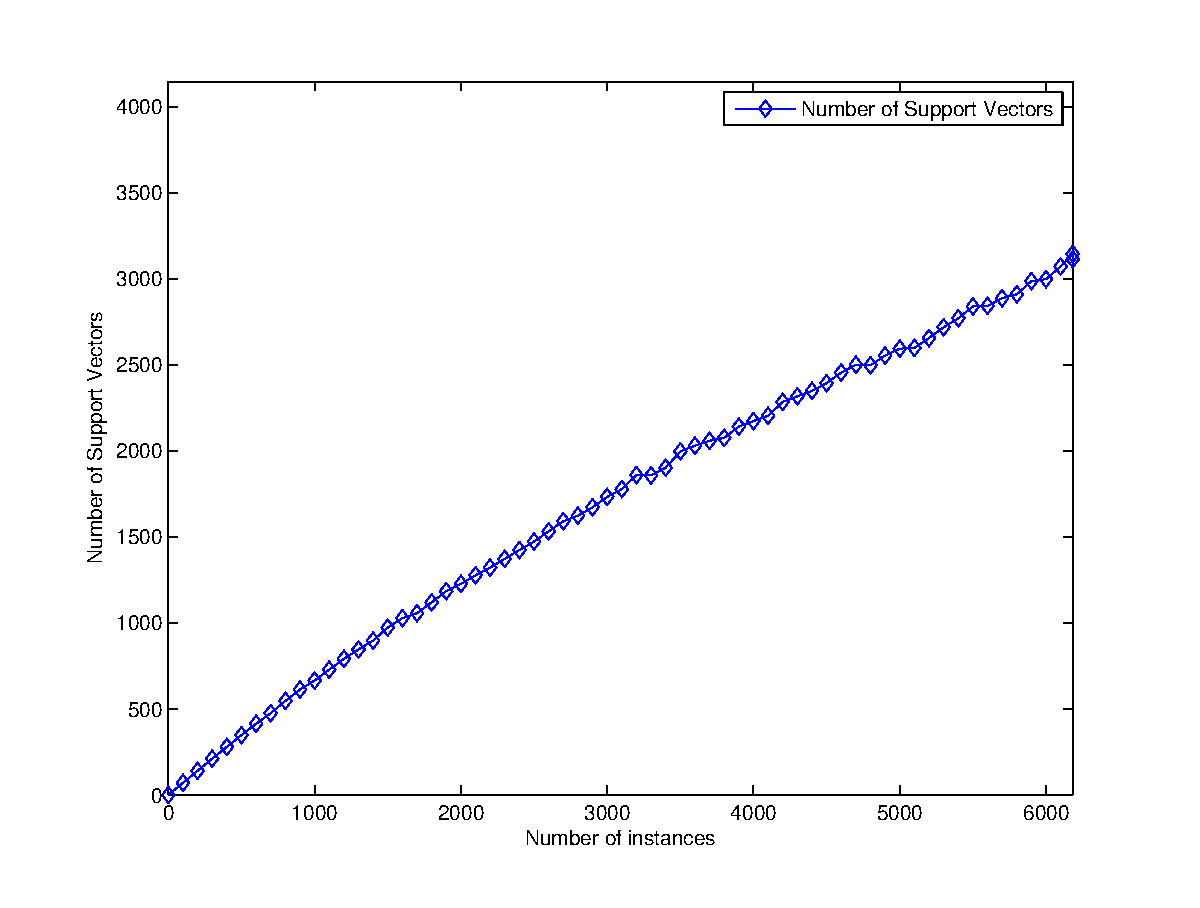
\includegraphics[width=0.8\textwidth]{svm_n_sv.eps}
    \caption{Variation of the number of support vectors in a linear kernel SVM, measured against the total number of instances}
    \label{fig:svm_n_sv}
\end{figure}

\subsection{Ensemble Learning}
Ensemble learning algorithms are essentially a combination of individual classifiers. In this work, these individual classifiers are support vector machines, which means that irrespective of which class of ensemble methods is used, the behavior is going to depend on the kernel being used. Since the maximum accuracy in the section on support vector machines was found with the linear kernel, the same is used in the following experiments. In all experiments presented in this section, except for measuring the accuracy of a bagging ensemble against the number of models, the total number of models comprising an ensemble is set to 9.

\subsubsection{Bagging}
The increase in the accuracy observed by a bagging based ensemble is similar to the increase observed in simple support vector machines. This can be attributed to the fact that bagging is essentially just a combination of SVM classifiers, with a majority vote deciding the final label of the instance. This can be observed in Figure~\ref{fig:bagging_accuracy}. A peak value of 79.97\% is observed when the ensemble has to classify 6000 data points. Similarly, when the classifier was trained on all 6182 points without any iterations, an average accuracy of 79.65\% was observed, which is a small improvement over the SVM classifier.\\

\begin{figure}
    \centering
    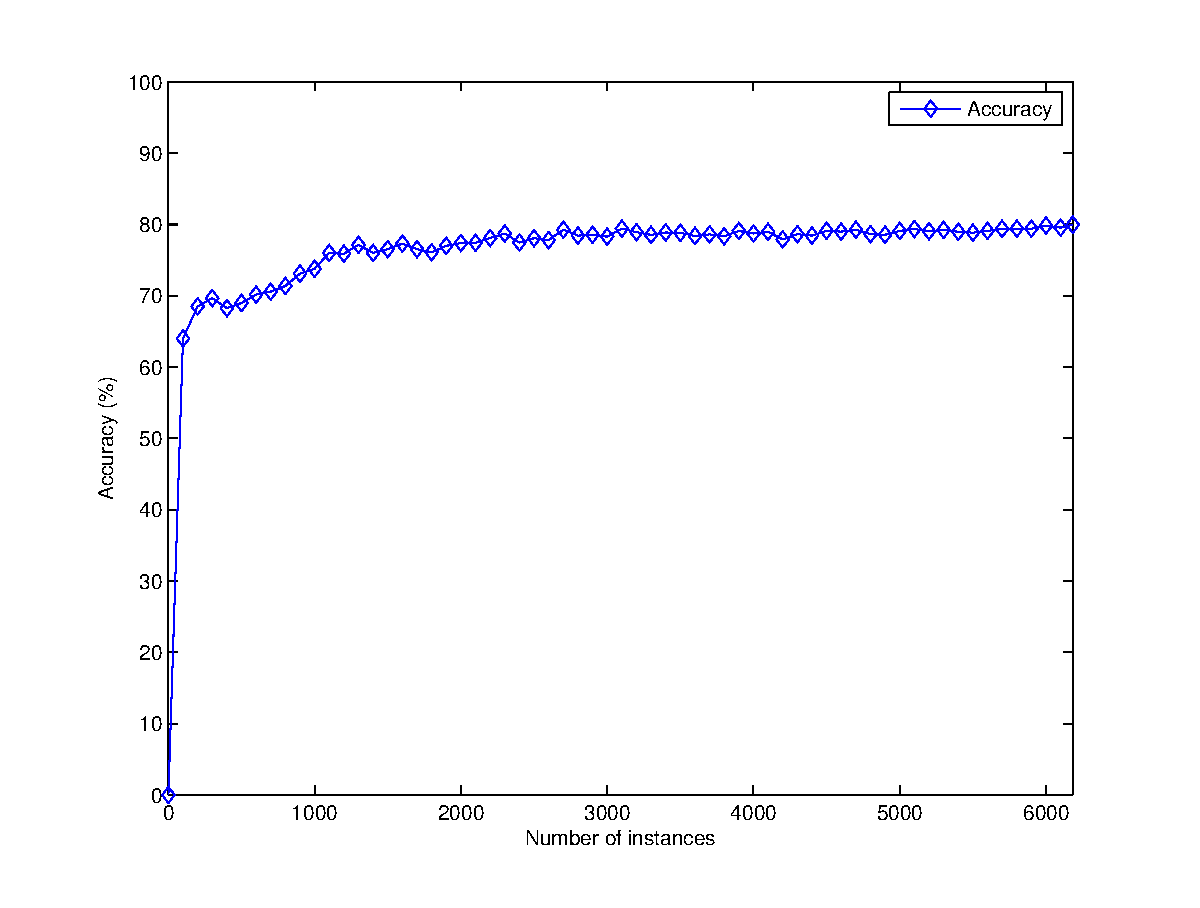
\includegraphics[width=0.8\textwidth]{bagging_accuracy.eps}
    \caption{Accuracy of a bagging ensemble (comprised of 9 linear kernel support vector machines) as measured against the number of instances}
    \label{fig:bagging_accuracy}
\end{figure}

On the other hand, Figure~\ref{fig:bagging_n_models} suggests that on varying the number of underlying classifiers from 1 to 20, the accuracy of a bagging based ensemble does not vary too much with the total number of models being used underneath. A maximum accuracy of 80.02\% is observed for 7 classifiers, while the minimum value is 73.66\% for 2 classifiers.

\begin{figure}
    \centering
    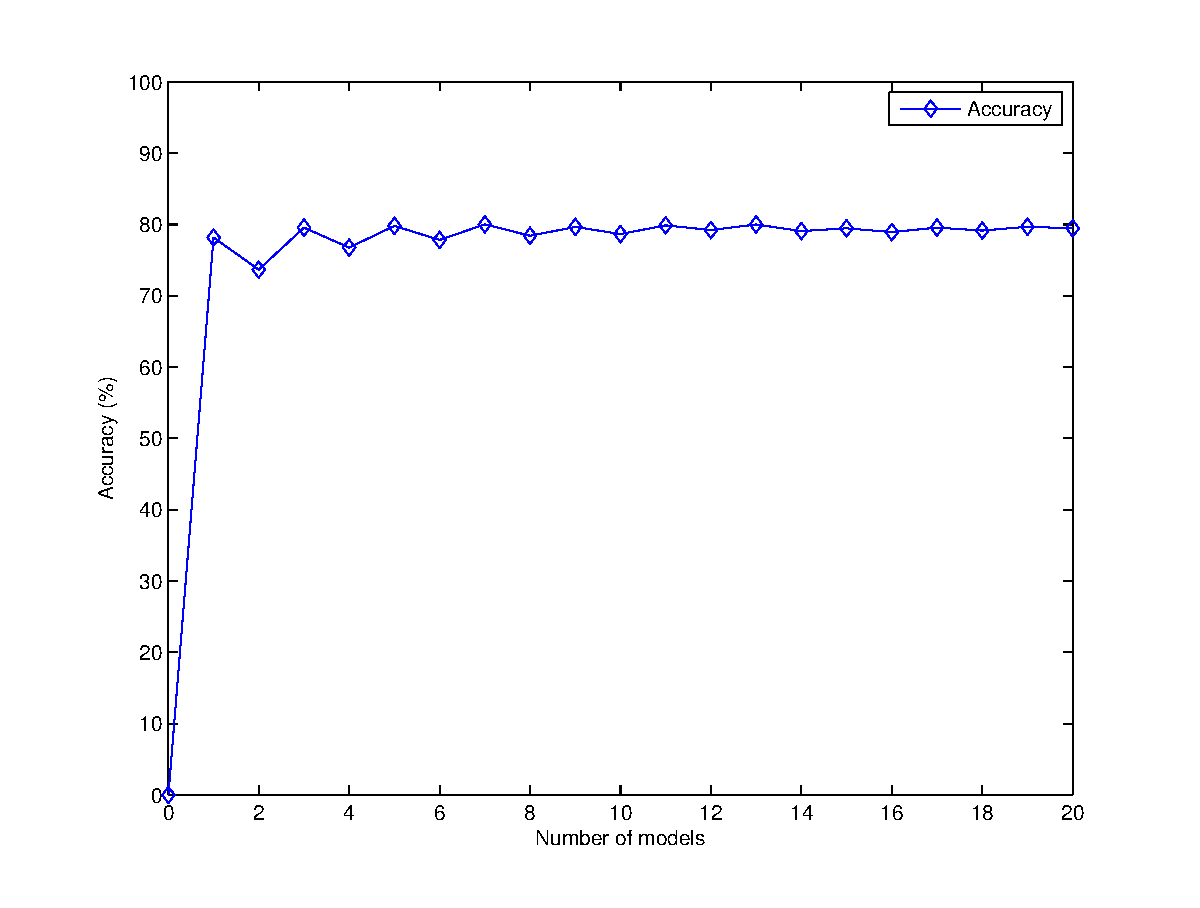
\includegraphics[width=0.8\textwidth]{bagging_n_models.eps}
    \caption{Variation of accuracy of a bagging ensemble with the number of constituent models}
    \label{fig:bagging_n_models}
\end{figure}

\subsubsection{Boosting}
Boosting follows a different approach to ensemble learning, by combining classifiers in a way that each successive classifier gets more incentive to classify correctly the points which the previous classifier misclassified. As shown in Figure~\ref{fig:boosting_accuracy}, the performance of a 9-classifier ensemble peaks at 78.66\%, and does not vary a lot as the number of instances increases. However, the average performance observed was 72.84\%, which is considerably less than that in case of support vector machines.

\begin{figure}
    \centering
    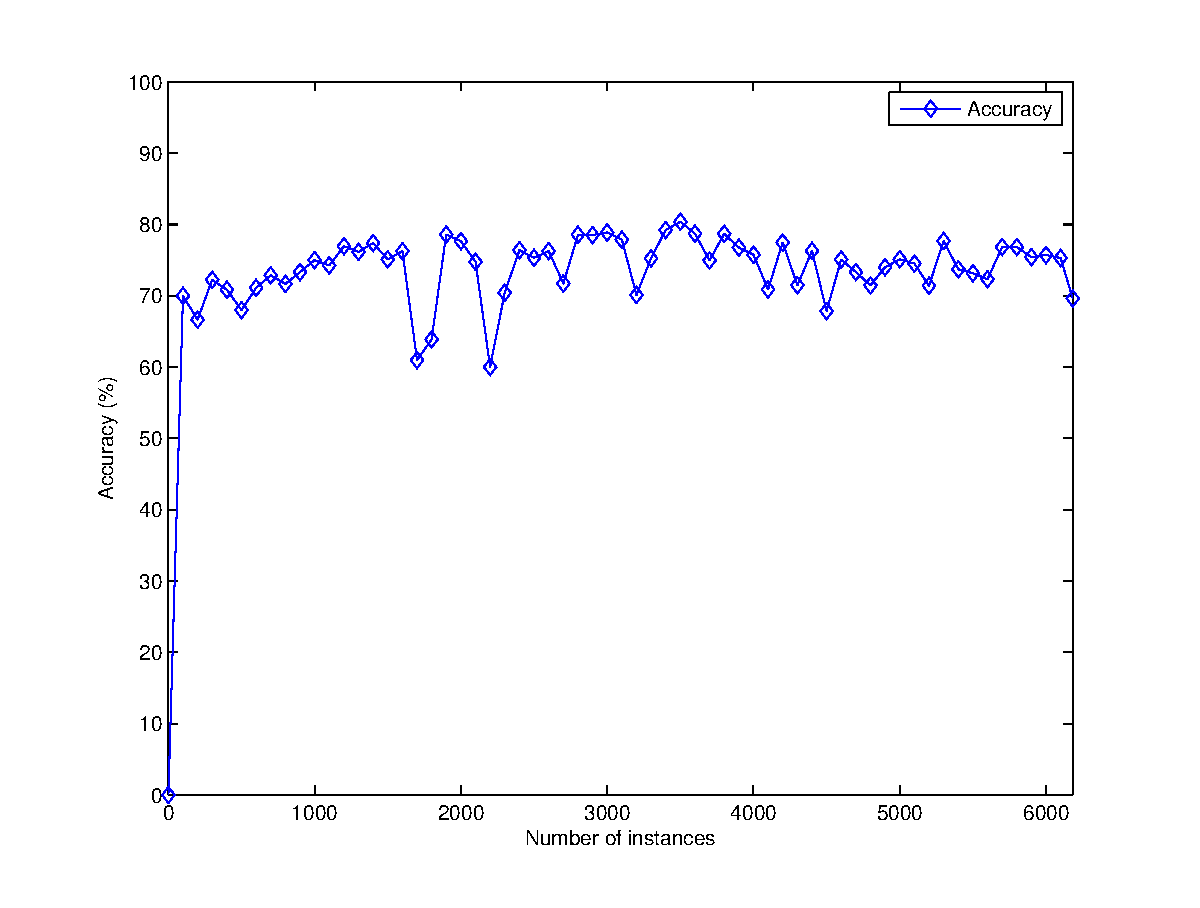
\includegraphics[width=0.8\textwidth]{boosting_accuracy.eps}
    \caption{Accuracy of a boosting ensemble (constituted by 9 linear kernel support vector machines) as measured against the number of instances}
    \label{fig:boosting_accuracy}
\end{figure}

\subsubsection{Stacking}
Stacking follows a more meta-level appraoch to classification, by training two levels of classifiers to perform the final classification. It can be seen in Figure~\ref{fig:stacking_accuracy} that the performance of stacked classifiers increases with the total number of instances, similar to the other two methods of ensemble learning. A maximum performance of 79.76\% is seen at the point when the model has to classify all 6182 instances, while the minimum (67\%) is seen when measurements are done on 100 instances. Similarly, when the classifier was trained on all 6182 instances without any iterations, an average accuracy of 79.48\% was observed, which is again a very small increase over the performance of a single support vector machine.

\begin{figure}
    \centering
    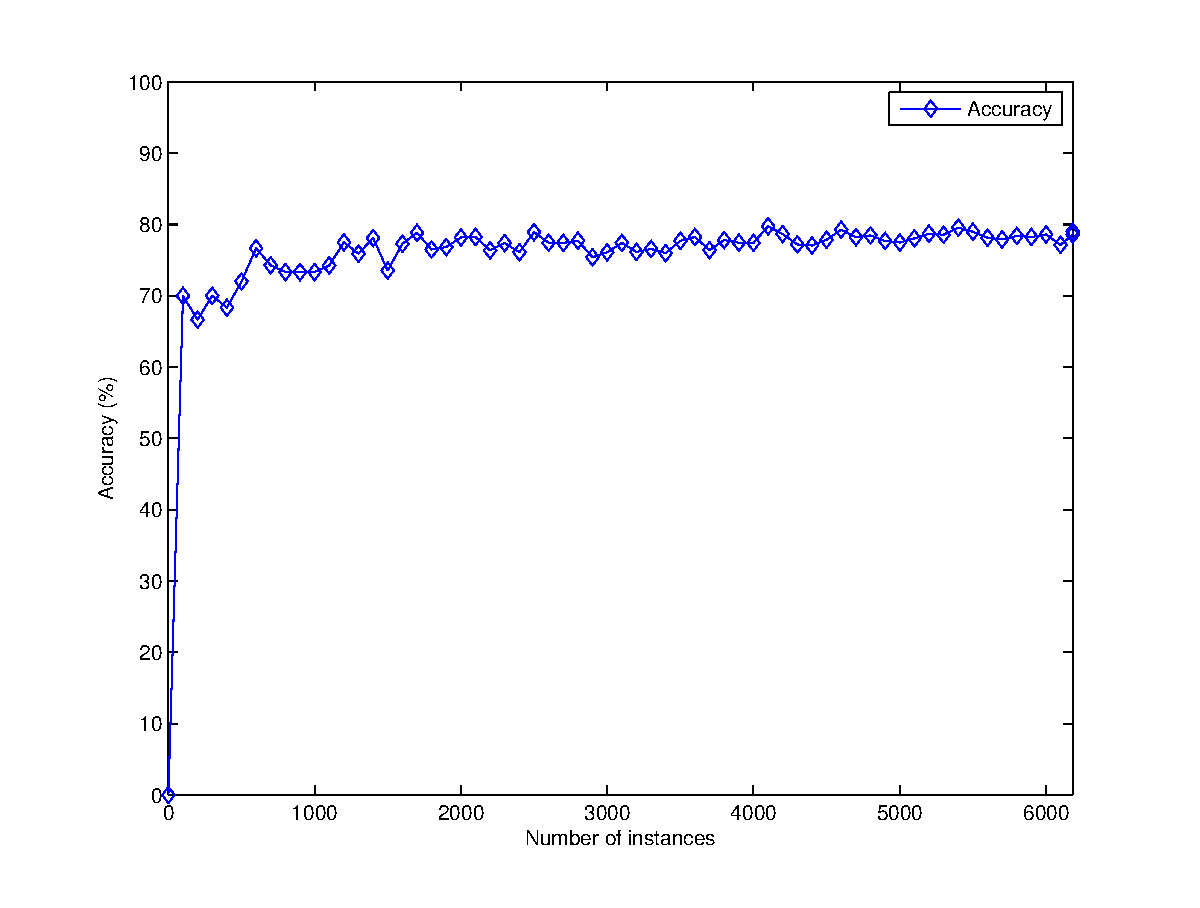
\includegraphics[width=0.8\textwidth]{stacking_accuracy.eps}
    \caption{Accuracy of linear kernel based stacking ensemble as measured against the number of instances}
    \label{fig:stacking_accuracy}
\end{figure}

\section{System Details}
\label{section:system_details}

The second major contribution of this thesis is a web based system that allows users to perform various functions including helping building the training data, evaluating a level of distress amongst the general public by monitoring the status of the classifier, and keeping a check on particular instances of content that may appear to be distressed and qualified as needing-attention.\\

Users help build the training data by assigning labels to stories fetched from Reddit. This accounts for the crowd intelligence part of the whole system, and constitutes the \emph{Ratings} module on the site. The \emph{Monitoring} module then uses this data to train the classifiers and present information about a general level of distress amongst people who are posting on Twitter (grouped by date) as monitored by each class of classifiers (SVM, Bagging, Boosting, and Stacking). The module also presents information about individual instances of content that are most likely to be depressed. This may then serve as a first step towards providing further attention (in the form of human help) to the authors of these tweets.\\

As soon as a user visits the front page of the web interface, they are presented with a choice between the \emph{Ratings} and \emph{Monitoring} modules, as shown in Figure~\ref{fig:landing}.\\

\begin{figure}
    \centering
    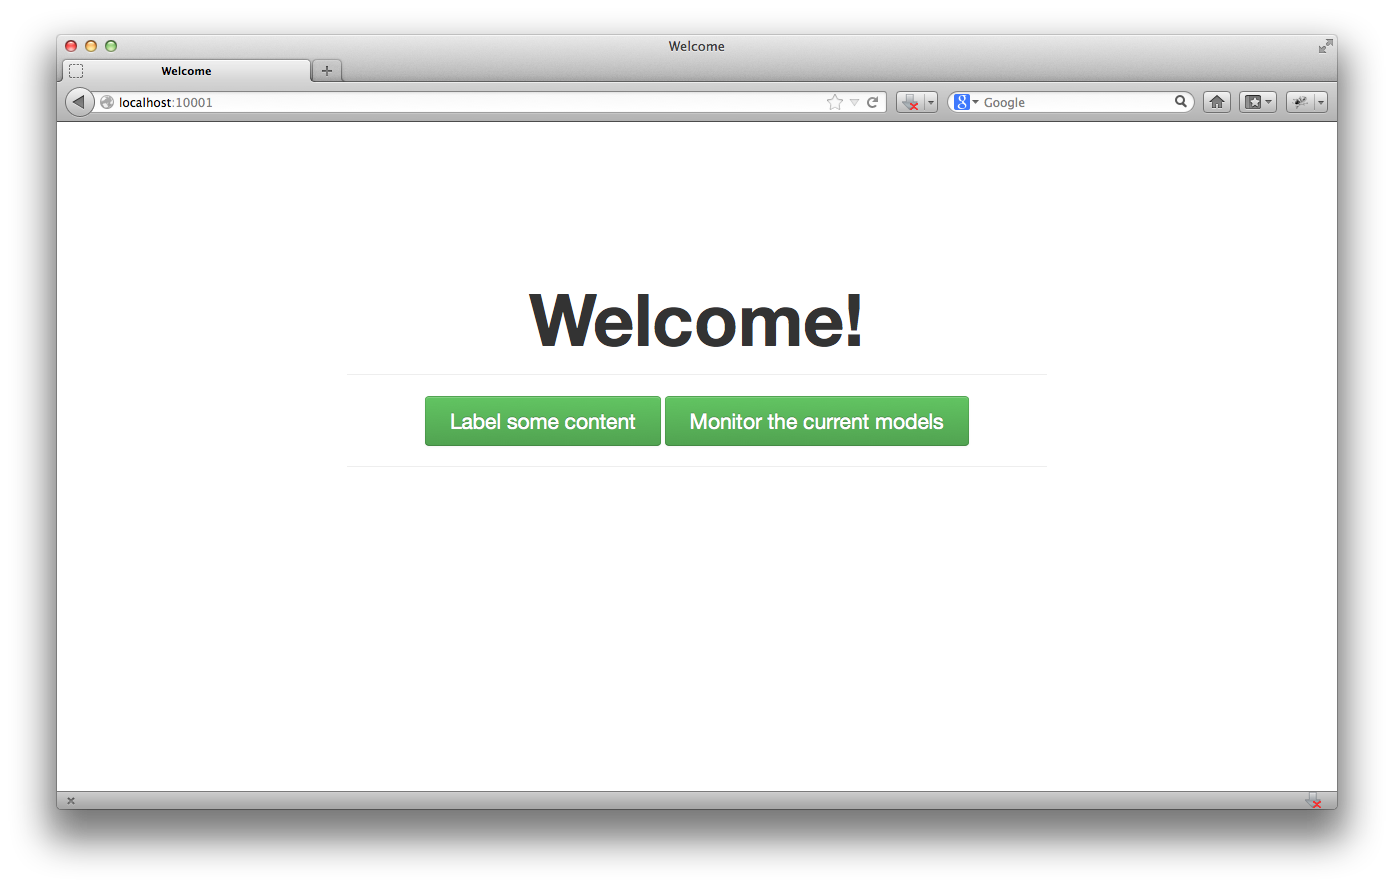
\includegraphics[width=0.8\textwidth]{landing.png}
    \caption{Landing page}
    \label{fig:landing}
\end{figure}

The division of the system into the two mentioned modules is from a user's perspective. From an infrastructure perspective, the system can be seen as being powered by two components, a manual one and an automatic one. The manual component includes users assigning labels to posts fetched from Reddit, which ultimately serves as the training data. The automatic component includes cron jobs (pieces of code that are executed at specific intervals of time) and involves fetching 800 tweets every day from the public stream of Twitter, collecting and consolidating statistics about the total number of depressed and not-depressed content posted each day, and updating the labels of all fetched tweets according to the updated models. In the next two sections, a discussion is presented about the system components from the user's perspective.

\subsection{Ratings}
The \emph{Ratings} module is built to help consolidate training data. As mentioned earlier, 1000 posts from Reddit are fetched every 2 days (500 each from \href{http://www.reddit.com/r/happy}{``/r/happy''}, and \href{http://www.reddit.com/r/suicidewatch}{``/r/suicidewatch''}), which do not contain any label information. As shown in Figure~\ref{fig:ratings}, this module presents a user with a random piece of text fetched from reddit, and two options for assigning this story a label. The label could be either ``depressed'', or ``not depressed''. If in case there are no unlabelled stories left, a simple message saying ``No unlabelled stories left'' is displayed.

\begin{figure}
    \centering
    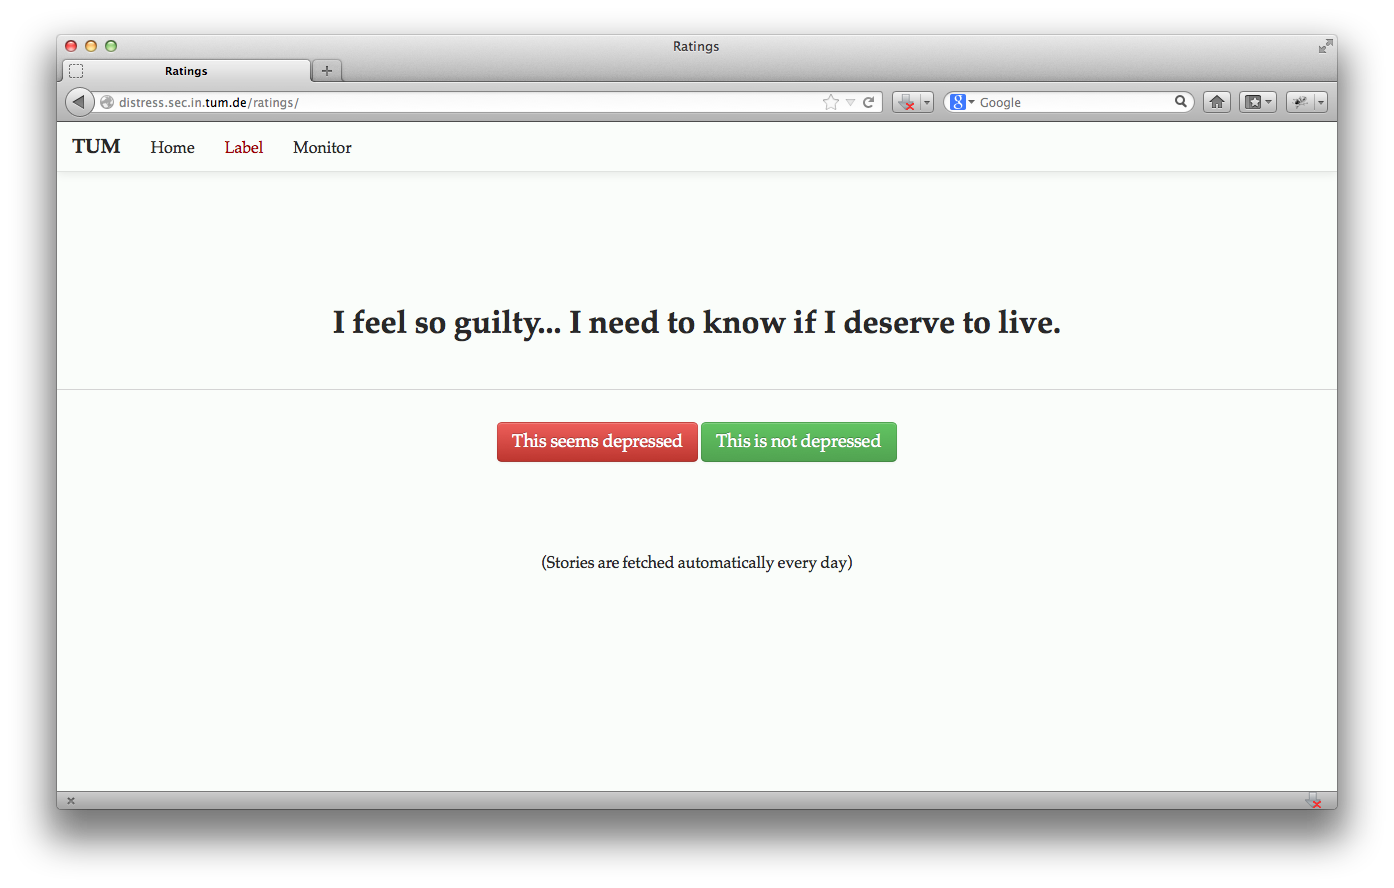
\includegraphics[width=0.8\textwidth]{ratings.png}
    \caption{Ratings module}
    \label{fig:ratings}
\end{figure}

\subsection{Monitoring}
The \emph{Monitoring} module is responsible for performing mainly two functions. The first function is to display a list of the top few tweets that are most likely to be depressed. This calculation is done based on the number of classifiers that classified a tweet as depressed. This is illustrated in Figure~\ref{fig:monitoring_landing_1} and Figure~\ref{fig:monitoring_landing_2}.\\

\begin{figure}
    \centering
    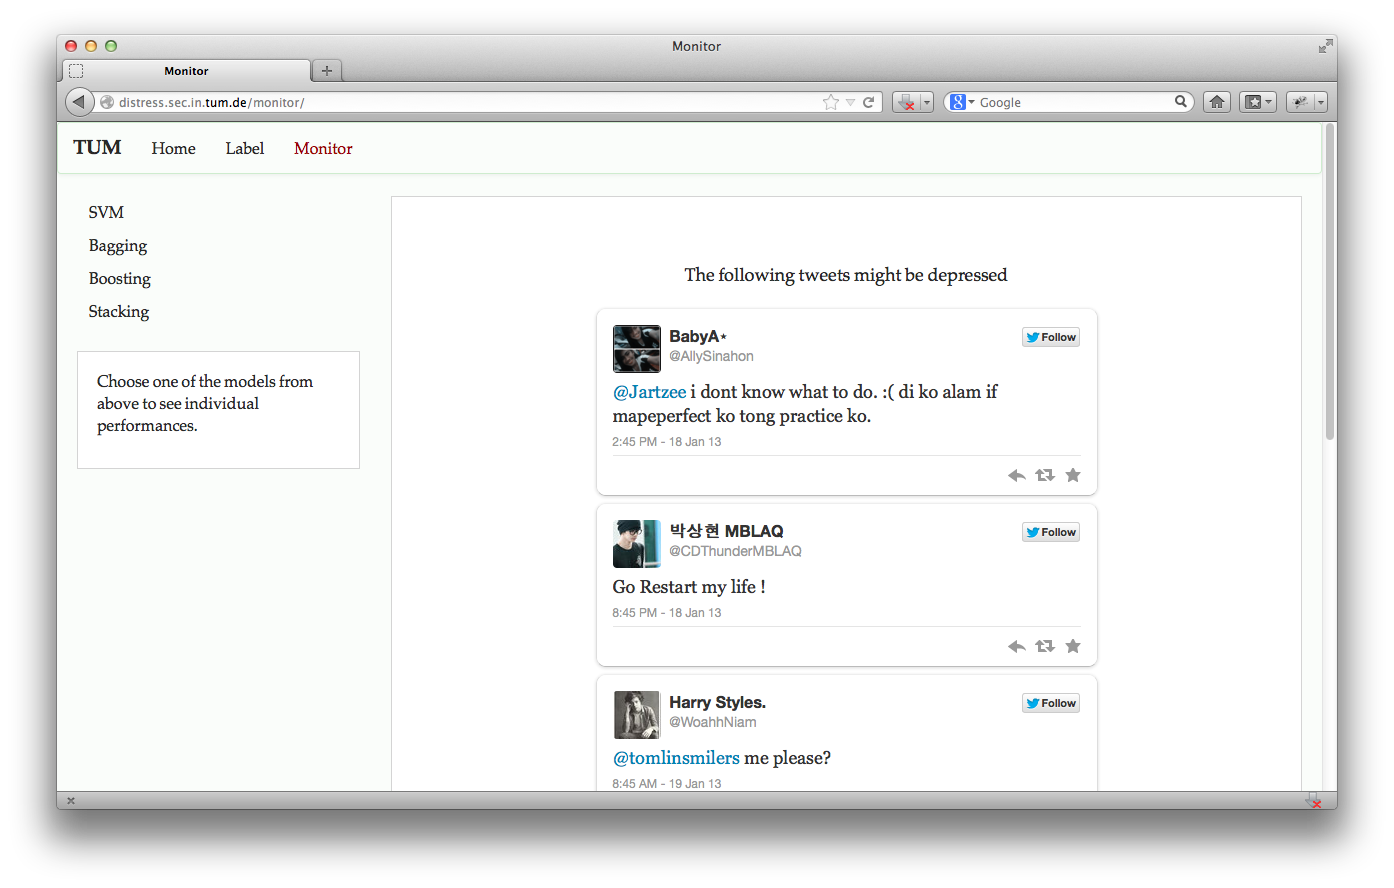
\includegraphics[width=0.8\textwidth]{monitoring_landing_1.png}
    \caption{Landing page of Monitoring module}
    \label{fig:monitoring_landing_1}
\end{figure}

\begin{figure}
    \centering
    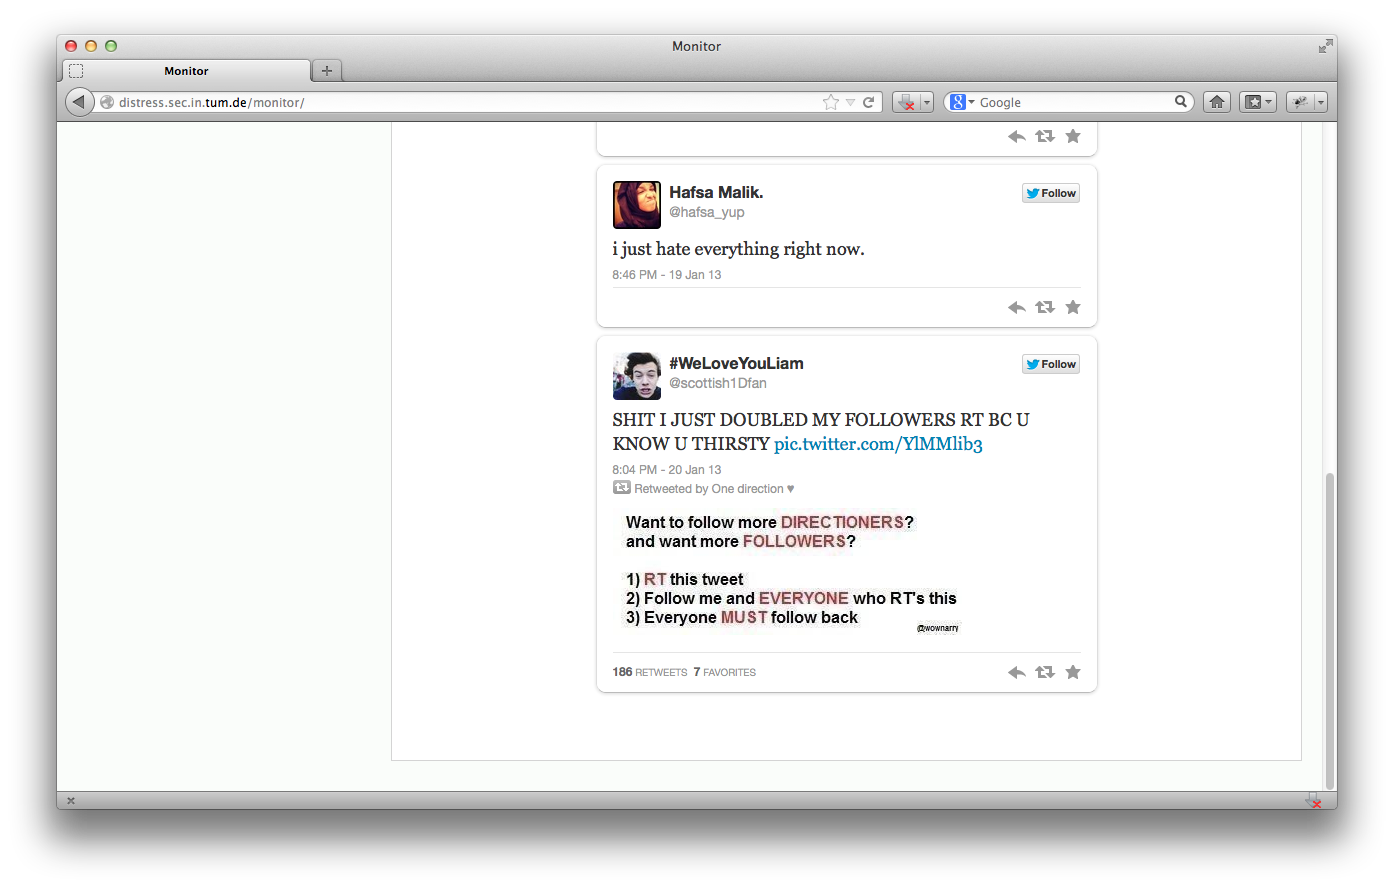
\includegraphics[width=0.8\textwidth]{monitoring_landing_2.png}
    \caption{Landing page of Monitoring module}
    \label{fig:monitoring_landing_2}
\end{figure}

As can be seen in Figure~\ref{fig:monitoring_landing_2}, one of the tweets displayed has the text \emph{``i just hate everything right now''}. Such content can be associated with feelings of resentment, and so this is a good candidate to pass on to a human for a final call on whether the person posting this is depressed or not. Similarly, Figure~\ref{fig:monitoring_landing_1} shows a tweet with the content that includes the phrase \emph{``i dont know what to do''}. A lot of content like this was found on \href{http://www.reddit.com/r/suicidewatch}{``/r/suicidewatch''}, where people often post when they feel confused in a very negative connotation. Hence, this tweet alone gives somewhat of an indication that this person might be feeling depressed, and this belief could be further solidifed (or not) after looking at the entire stream of this person.\\

The second function that the \emph{Monitoring} module performs is that of displaying statistics about how many tweets were classified as depressed on a particular day. Figure~\ref{fig:monitoring_bagging} shows the page that is displayed when a user chooses to view the statistics for the bagging classifier.\\

\begin{figure}
    \centering
    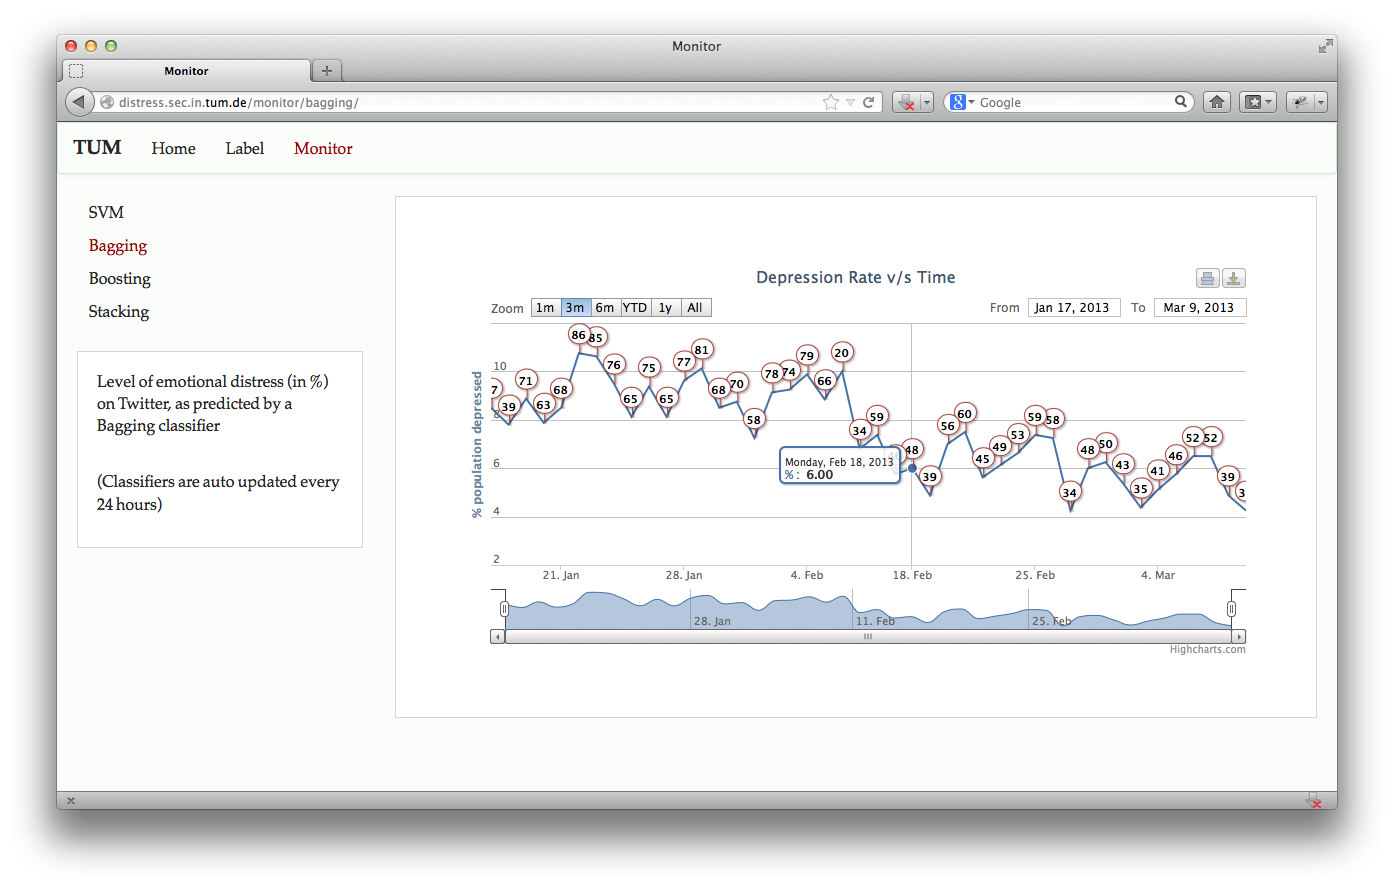
\includegraphics[width=0.8\textwidth]{monitoring_bagging.png}
    \caption{Statistics for the bagging classifier}
    \label{fig:monitoring_bagging}
\end{figure}

As can be seen in the figure, the statistics are displayed for a time period beginning from January 17 (this is when the process of collecting tweets from Twitter began) until March 18, with intervals of 15 days between two consecutive sections in the graph. The graph can also be zoomed in on a smaller period of time, as shown in Figure~\ref{fig:monitoring_bagging_zoomed}, in which case only the statistics for that period of time are displayed. The zoom level can be reset using the \emph{``Reset Zoom''} button.

\begin{figure}
    \centering
    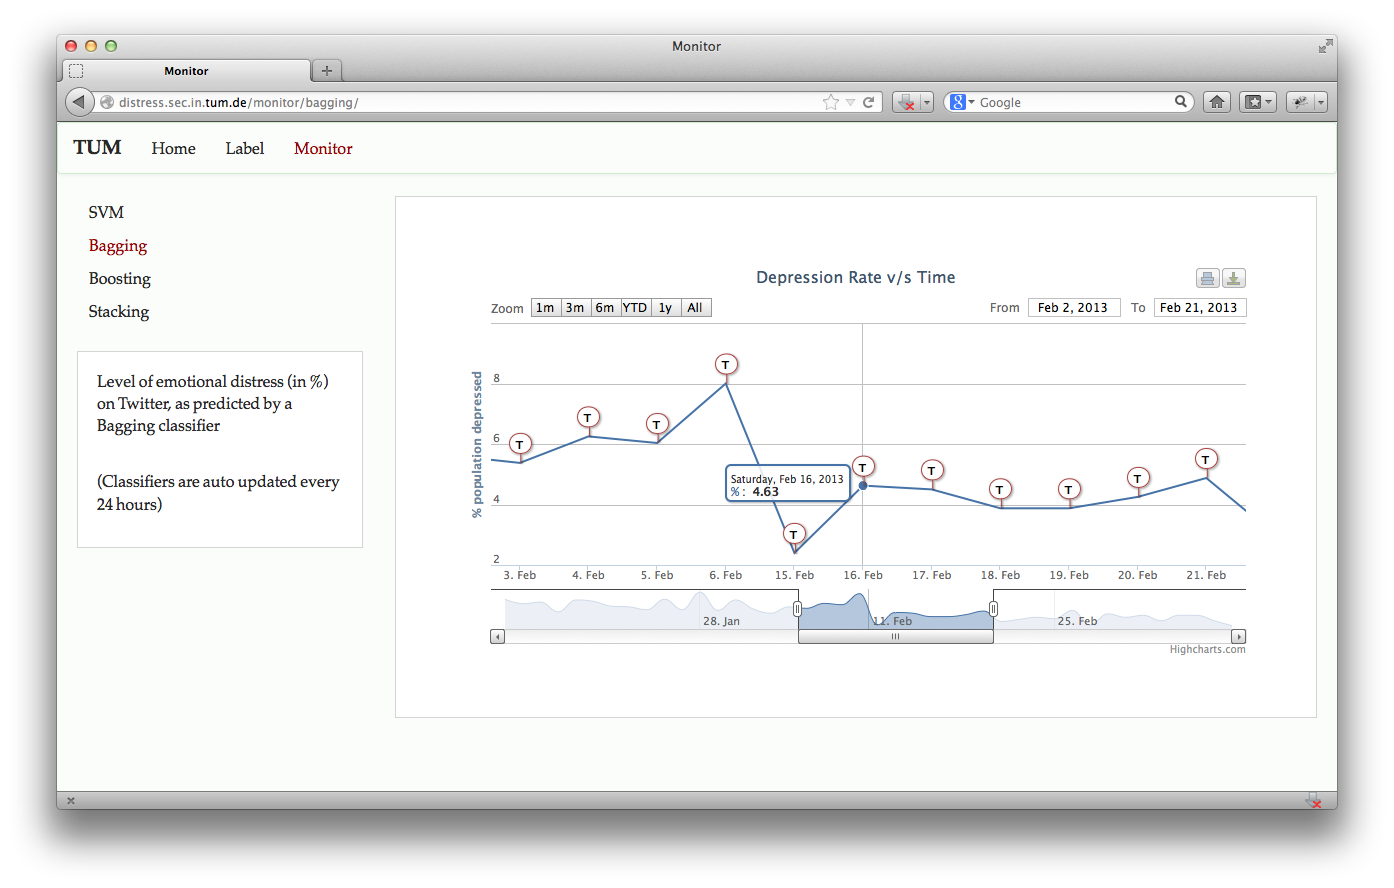
\includegraphics[width=0.8\textwidth]{monitoring_bagging_zoomed.png}
    \caption{Zooming in on a particular interval of time for Bagging statistics}
    \label{fig:monitoring_bagging_zoomed}
\end{figure}
